\chapter{Упругость и энергия несоответствия}

Эта глава --- сердце задачи о гидридах. Гидрид объёмнее матрицы на 17\,\%, и металл вокруг него вынужден
деформироваться. Энергия этой деформации определяет, какой формы будет пластинка, в какой плоскости она ляжет,
почему нужен переохлаждённый раствор и как на всё это влияет внешняя нагрузка.

\section{Напряжения и деформации}

\textbf{Деформация} описывает, как меняются расстояния между точками тела. Если точка $\mathbf x$ сместилась на
$\mathbf u(\mathbf x)$, тензор малых деформаций
\begin{equation}
\eps_{ij} = \tfrac12\Bigl(\frac{\partial u_i}{\partial x_j} + \frac{\partial u_j}{\partial x_i}\Bigr).
\end{equation}
Диагональные компоненты --- относительные удлинения вдоль осей, недиагональные --- половины углов сдвига.
След $\eps_{kk}$ --- относительное изменение объёма.

\textbf{Напряжение} $\sigma_{ij}$ --- сила на единицу площади: $j$-я компонента силы, действующей на площадку с
нормалью вдоль $i$. Тензор симметричен. Его удобно разложить на \textbf{гидростатическую} часть
$\sigma_h = \sigma_{kk}/3$ (всестороннее растяжение или сжатие --- оно меняет объём и влияет на растворённый
водород, глава~3) и \textbf{девиатор} $s_{ij} = \sigma_{ij} - \sigma_h\delta_{ij}$ (формоизменение --- оно
двигает дислокации, глава~7).

Для изотропного тела закон Гука
\begin{keyf}[Закон Гука]
\[
\sigma_{ij} = \lambda\,\eps_{kk}\,\delta_{ij} + 2\mu\,\eps_{ij},\qquad
E = \frac{\mu(3\lambda+2\mu)}{\lambda+\mu},\quad \nu = \frac{\lambda}{2(\lambda+\mu)},\quad K = \lambda + \tfrac23\mu ,
\]
плотность упругой энергии $w = \tfrac12\sigma_{ij}\eps_{ij}$.
\end{keyf}
Для циркония при 300--400\degC{} $E\approx 80$--$90$~ГПа, $\nu\approx0.34$, $\mu\approx30$--$33$~ГПа. На самом деле
монокристалл Zr заметно анизотропен; изотропное приближение даёт верные порядки и большинство качественных
выводов.

\section{Собственная деформация}

Нагрейте свободный стержень --- он удлинится на $\alpha\Delta T$, но напряжений не будет. Зажмите его концы и
нагрейте снова --- длина не изменится, зато появится сжатие $\sigma = -E\alpha\Delta T$. Удлинение $\alpha\Delta T$,
которое материал «хочет» иметь, называют \textbf{собственной деформацией} $\eps^*$. Напряжение создаёт только
разница между фактической и собственной деформацией:
\begin{equation}
\sigma_{ij} = C_{ijkl}\,\bigl(\eps_{kl} - \eps^*_{kl}\bigr).
\end{equation}
Превращение матрицы в гидрид --- то же самое: кусочек металла «хочет» стать больше на $\eps^*$ (4.6\,\% в
базисной плоскости и 7.2\,\% вдоль $c$), а окружающий металл ему не даёт.

\section{Задача Эшелби}

Эшелби (1957) решил эту задачу с помощью мысленного опыта из четырёх шагов (рис.~\ref{fig:f5_eshelby}):
\begin{enumerate}
\item вырежем из бесконечного тела область $\Omega$ --- будущее включение;
\item дадим ей свободно превратиться: она примет собственную деформацию $\eps^*$ без напряжений;
\item приложим к её поверхности силы, которые вернут ей исходную форму (напряжение внутри $-\mathbf C:\eps^*$),
  и вставим обратно;
\item уберём силы --- точнее, приложим к поверхности противоположные. Тело деформируется и придёт в равновесие:
  напряжения появятся и внутри включения, и вокруг него.
\end{enumerate}

\fig{f5_eshelby}{Мысленный опыт Эшелби: вырезать, свободно превратить, сжать до исходной формы и вставить,
отпустить. Последний шаг --- обычная задача теории упругости о силах на поверхности.}

Главный результат Эшелби: \textbf{если включение --- эллипсоид, то деформация внутри него однородна} и линейно
выражается через $\eps^*$: $\eps = \mathbf S:\eps^*$, где тензор Эшелби $\mathbf S$ зависит только от формы
эллипсоида и коэффициента Пуассона. Упругая энергия
\begin{equation}
W = -\tfrac12\,V\,\sigma^{\text{вн}}_{ij}\,\eps^*_{ij},
\end{equation}
где $\sigma^{\text{вн}}$ --- напряжение внутри включения. В частности, для шара с чистым расширением
$\eps^* = \eps\,\mathbf I$ при одинаковых упругих константах включения и матрицы
\begin{keyf}[Шар с несоответствием]
\[
W = \frac{2\mu(1+\nu)}{1-\nu}\,\eps^2\,V = \frac{E}{1-\nu}\,\eps^2\,V .
\]
\end{keyf}

\begin{idea}
Удивительный факт: для чистого расширения эта энергия \emph{не зависит от формы} эллипсоида --- шар, игла и диск
стоят одинаково. Матрица вокруг расширяющегося включения деформируется так, что выигрыш в одном направлении
компенсирует проигрыш в другом. Форма начинает играть роль, только когда несоответствие \emph{анизотропно} (как у
гидрида) или упругие константы включения и матрицы различаются.
\end{idea}

\section{Тонкая пластинка: почему гидриды плоские и где они ложатся}

Пусть включение --- очень тонкая пластинка с нормалью $\mathbf n$. Поперёк пластинки ей ничто не мешает
расшириться: тонкий слой может свободно сдвинуть окружающий металл, почти не деформируя его. А вот в плоскости
пластинки матрица держит её жёстко --- там включение вынуждено иметь ту же длину, что и матрица. Значит,
упругую энергию дают только деформации \emph{в плоскости} пластинки. Если $t$ и $s$ --- два направления в плоскости
пластинки,
\begin{keyf}[Энергия тонкой пластинки]
\[
\frac{W}{V} = \frac{E}{2(1-\nu^2)}\Bigl(\eps^{*2}_{tt} + \eps^{*2}_{ss} + 2\nu\,\eps^*_{tt}\eps^*_{ss}\Bigr) + 2\mu\,\eps^{*2}_{ts} .
\]
Компоненты $\eps^*_{nn}$, $\eps^*_{nt}$, $\eps^*_{ns}$ (поперёк пластинки) энергии не стоят.
\end{keyf}

Для гидрида это решает ориентацию пластинки:
\begin{itemize}
\item пластинка на базисной плоскости: в плоскости --- две «малые» деформации по 4.6\,\%, а большая (7.2\,\%)
  поперёк и ничего не стоит. $W/V = E\eps_a^2/(1-\nu) \approx 286$~МДж/м$^3$;
\item пластинка, параллельная оси $c$: в её плоскость попадает большая деформация 7.2\,\%,
  $W/V\approx 487$~МДж/м$^3$, на 70\,\% больше.
\end{itemize}
Гидриду выгодно лечь так, чтобы самое большое расширение было направлено поперёк пластинки: \textbf{около
базисной плоскости}. На рис.~\ref{fig:f5_orient}а энергия показана для всех наклонов. Наблюдаемая плоскость
$\{10\bar17\}$ отклонена от базиса на 15\textdegree; в изотропном приближении это стоит всего 4\,\% лишней энергии,
а точный выбор плоскости задают уже анизотропия упругости и строение границы.

\fig{f5_orient}{а) Упругая энергия тонкой пластинки $\delta$-гидрида на единицу объёма (и на моль водорода, правая
шкала) от угла между нормалью пластинки и осью $c$ ($E = 90$~ГПа, $\nu = 0.34$). Минимум --- на базисной
плоскости; пунктир --- плоскость $\{10\bar17\}$. б) Работа приложенного растяжения на несоответствии гидрида
$\sigma\eps^*_{xx}$ от угла между осью $c$ зерна и направлением растяжения: больше всего --- у зёрен с осью $c$
вдоль нагрузки. Заметьте масштабы: на панели а --- сотни, на панели б --- единицы МДж/м$^3$.}

Как энергия переходит от шара к пластинке, показывает расчёт на рис.~\ref{fig:f5_shape}. Он сделан тем же
методом Фурье, что в модели (раздел~\ref{sec:fourier}), для эллиптических включений в плоской деформации. Для
чистого расширения энергия от формы не зависит (в пределах 1\,\% погрешности сетки). Для несоответствия гидрида
пластинка на базисе с утоньшением дешевеет, а пластинка вдоль $c$ дорожает. Обе стремятся к пределам тонкой
пластинки из формулы выше.

\begin{figure}[htbp]\centering
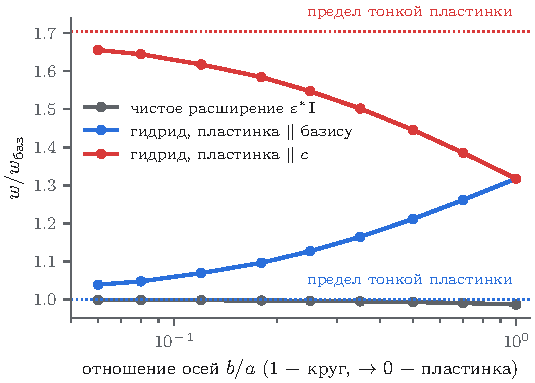
\includegraphics[width=0.66\linewidth]{f5_shape}
\caption{Упругая энергия эллиптического включения на единицу объёма от отношения осей, в единицах энергии тонкой
базисной пластинки. Точки --- расчёт методом Фурье (сетка $1024^2$). Серые --- чистое расширение: энергия от формы не
зависит, как и предсказывает Эшелби. Синие и красные --- несоответствие гидрида для пластинки, параллельной
базису и оси $c$; пунктир --- пределы тонкой пластинки.}
\label{fig:f5_shape}
\end{figure}

\section{Поле вокруг пластинки}

Внутри пластинки напряжения огромны --- гигапаскали (порядка $E\eps^*$). Но для соседей важнее поле \emph{снаружи}
(рис.~\ref{fig:f5_field}). Пластинка расширяется поперёк себя и раздвигает металл, как клин. Перед её торцами
матрица растянута: гидростатическое напряжение здесь доходит до сотен МПа. Над и под широкими гранями матрица
сжата.

\fig[0.75]{f5_field}{Гидростатическое напряжение в матрице вокруг тонкой пластинки $\delta$-гидрида (отношение
осей 0.1, нормаль вдоль $c$; расчёт методом Фурье, $E = 90$~ГПа). Красное --- растяжение, синее --- сжатие. У
торцов --- растяжение в сотни МПа.}

\begin{zrbox}
У торцов пластинки сходятся сразу два эффекта: туда стекается водород (глава~3), и там новой пластинке той же
ориентации выгоднее появиться --- её несоответствие «встраивается» в уже растянутую матрицу. Поэтому гидриды
растут цепочками торец к торцу, и из микропластинок складываются длинные макрогидриды. Над и под пластинкой
матрица сжата, и новые пластинки там зарождаются хуже. Насколько сильно одни пластинки влияют на зарождение
других --- один из ключевых и плохо известных параметров модели.
\end{zrbox}

\section{Работа внешнего напряжения}

Если тело нагружено однородным напряжением $\sigma^A$, появление включения меняет энергию системы дополнительно на
\begin{keyf}[Энергия взаимодействия с нагрузкой]
\[
\Delta G_{\text{вз}} = -\,\sigma^A_{ij}\,\eps^*_{ij}\,V .
\]
\end{keyf}
Этот результат тоже принадлежит Эшелби. Он точный и \emph{не зависит от формы} включения. Смысл простой:
нагрузка совершает работу на деформации превращения. Если включение расширяется вдоль растягивающей нагрузки,
работа положительна, и превращение облегчается.

Несоответствие гидрида связано с решёткой зерна, а не с формой пластинки. Поэтому нагрузка выбирает не форму, а
\emph{зёрна}: выгоднее всего выпадать в зёрнах, где ось $c$ (направление самого большого расширения, 7.2\,\%)
смотрит вдоль растяжения (рис.~\ref{fig:f5_orient}б). Пластинка в таком зерне лежит около базиса, то есть
\emph{поперёк} нагрузки. Именно так окружное напряжение в трубе рождает радиальные гидриды --- в тех зёрнах, чьи оси
$c$ близки к окружному направлению.

\begin{zrbox}
Сравним числа. Работа окружного напряжения 100~МПа: $\sigma\eps_c \approx 7$~МДж/м$^3$, то есть около 70~Дж на моль
водорода. Разница между лучшим и худшим зерном, $\sigma(\eps_c-\eps_a)$, --- всего 27~Дж/моль. Упругая
энергия самой пластинки --- около 3000~Дж/моль, движущая сила выпадения --- около 5000~Дж/моль. Нагрузка ---
поправка в один-два процента. Как такая малая поправка решает ориентацию, объясняет теория зарождения: работа
нагрузки входит в показатель экспоненты (глава~6).
\end{zrbox}

\section{Метод Фурье: как считает модель}
\label{sec:fourier}

Для многих пластинок произвольной формы аналитического решения нет. Его даёт метод, развитый Хачатуряном. Пусть
собственная деформация задана на периодической сетке: $\eps^*(\mathbf x) = \eps^{*0}\chi(\mathbf x)$, где $\chi$
равна 1 в гидриде и 0 в матрице. Уравнение равновесия $\partial_j\sigma_{ij} = 0$ с законом Гука после
преобразования Фурье становится \emph{алгебраическим}: для каждой гармоники $\mathbf k$
\begin{equation}
\hat{\mathbf u}(\mathbf k) = -i\,\mathbf N(\mathbf k)\,\bigl(\mathbf k\cdot\hat{\boldsymbol\tau}(\mathbf k)\bigr),
\qquad \hat{\boldsymbol\tau} = \mathbf C:\hat{\eps}^*,
\end{equation}
где $\mathbf N(\mathbf k) = (\mathbf k\cdot\mathbf C\cdot\mathbf k)^{-1}$ --- обратный «акустический» тензор. Для
изотропной среды
$N_{ij} = \dfrac{1}{\mu k^2}\Bigl(\delta_{ij} - \dfrac{\lambda+\mu}{\lambda+2\mu}\,n_in_j\Bigr)$, $\mathbf n = \mathbf k/k$.
Решение --- одно прямое и одно обратное быстрое преобразование Фурье, за $O(N\log N)$ операций для $N$ точек сетки.

У этого подхода есть красивое следствие. Упругая энергия выражается через форму включения и функцию направления
$B(\mathbf n)$:
\[
W = \frac{1}{2}\int B(\mathbf n)\,|\hat\chi(\mathbf k)|^2\,\frac{\dd^3k}{(2\pi)^3},\qquad
B(\mathbf n) = \boldsymbol\sigma^0:\eps^{*0} - \mathbf n\cdot\boldsymbol\sigma^0\cdot\mathbf N(\mathbf n)\cdot\boldsymbol\sigma^0\cdot\mathbf n,
\]
где $\boldsymbol\sigma^0 = \mathbf C:\eps^{*0}$. У тонкой пластинки спектр $\hat\chi$ сосредоточен вдоль её нормали,
и энергия на объём равна $B(\mathbf n)$ при нормали пластинки. Значит, \textbf{плоскость залегания --- та, чья нормаль
минимизирует $B(\mathbf n)$}. Это правило Хачатуряна; формула тонкой пластинки выше --- его частный случай.

\begin{exercise}
Повторите вывод энергии шара: внутри шара с чистым расширением полная деформация
$\eps^{\text{вн}} = \frac{1+\nu}{3(1-\nu)}\eps\,\mathbf I$. Найдите напряжение внутри и подставьте его в
$W = -\tfrac12 V\sigma^{\text{вн}}:\eps^*$.
\end{exercise}

\begin{exercise}
Выведите формулу энергии тонкой пластинки, считая, что в её плоскости полная деформация равна нулю, а поперёк
напряжения нет (плоское напряжённое состояние в пластинке).
\end{exercise}

\begin{exercise}
Посчитайте энергию тонкой пластинки для нормали под 15\textdegree{} к оси $c$. Сколько это на моль водорода, если
объём гидрида на моль водорода $10^{-5}$~м$^3$?
\end{exercise}

\begin{exercise}
Окружное напряжение 120~МПа, осевое 60~МПа (труба с заглушками). Найдите работу $\sigma^A:\eps^*$ на моль водорода для
зерна, у которого ось $c$ лежит вдоль окружного направления, и для зерна с осью $c$ по радиусу.
\end{exercise}
